\chapter{Methylorubrum extorquens\authorB{}}

\section{{Taxonomy}}

\subsection{Phylum Pseudomonia}
Pseudomonadota is a major phylum of Gram-negative bacteria (information about Gramnegative bacteria will follow further down). They are incredibly diverse, encompassing
pathogens, free-living species, nitrogen-fixing bacteria, and many more.
Pseudomonadota exhibit a large range of shapes and sizes as well as metabolisms and
habitats which will also be discussed further down. The diversity of Pseudomonadota
makes them play a major role in the world's nutrient cycling ranging from crucial
ecological relationships with humans to simple things such as nitrogen fixation.
Pseudomonadota includes 5 classes but only the class Alphaproteobacteria is of
importance for us~\cite{pseudomonadota}.

\subsection{Class Alphaprotoebacteria}
Alphaproteobacteria is a highly diverse class of bacteria belonging to the phylum
Pseudomonadota.
They are named after the first letter of the Greek alphabet (alpha) due
to being one of the first major lineages to diverge within the proteobacteria phylum.

This class is incredibly varied, encompassing bacteria with a range of lifestyles including
phototrophs (light-using), methanotrophs (methane-utilizing), symbionts (mutually
beneficial relationships with other organisms), and pathogens (disease-causing).

Soil, Water including cold deep-sea vents, hot springs, and symbiotic relationships even
with humans are natural habitats of Proteobacteria~\cite{gammaproteobacteria}.

\textbf{Rhizobium:} These bacteria form a symbiotic partnership with legumes, such as peas and
soybeans.
Rhizobium colonizes the legume's root nodules and fixes atmospheric nitrogen
into a usable form that is essential for plant growth.

\textbf{Wolbachia:} This widespread genus of bacteria lives symbiotically within insects and other
arthropods.
Wolbachia can manipulate the host's reproduction in various ways,
sometimes even influencing sex ratios or protecting the host from viruses.

\textbf{Rickettsia:} This genus includes several species that are obligate intracellular pathogens,
meaning they can only live and reproduce inside the cells of a host organism. Rickettsiae
causes various human diseases, including typhus fever and Rocky Mountain spotted fever.

\textbf{Magnetococcus:} These magnetotactic bacteria contain magnetosomes, specialized
organelles that allow them to align and move along magnetic fields.

\subsection{Order Hyphomicrobiales}
Hyphomicrobiales can utilize single-carbon compounds like methanol as an energy
source, the bacterium Methylorubrum Extorquens does this for example.
Hyphomicrobiales produce carotenoid pigments and therefore appear pink or orange in
colonies. These colonies are aerobic which means they require oxygen for growth. They
inhabit a large variety of environments including soils, plant surfaces, root structures,
water, and dust.
They also play important ecological roles in their habitats, like plant-microbe interactions
when metabolizing methanol on plant leaves or carbon and nitrogen cycling in various
environments~\cite{methylobacteria_groups}.

\subsection{Genus Methylorubrum}
They use specialized pathways to break down methanol for energy and to create
biomass. This metabolic capability has potential applications in Bioremediation which
means that this bacteria can clean up methanol-contaminated areas. This family of
bacteria is also able to produce valuable chemicals from methanol~\cite{new_methylorubrum}.
Bacteria of the genus Methylorubrum are rod-shaped or slightly bent and show pink or
orange pigmentation like every genus that belongs to the order Methylobacterium.

\begin{figure}[H]
    \centering
    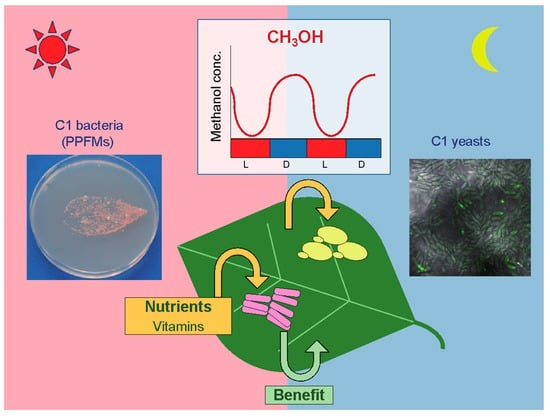
\includegraphics[width=0.8\textwidth]{./media/images/mextorquens_on_leaf}
    \caption{Pink \emph{Methylorubrum extorquens} on a leaf utilizing the plant's nutritiens.}
    \label{fig:mextorquens_on_leaf}
\end{figure}

\subsection{Species Extorquens}
In our thesis, the Extorquens bacterium species holds immense significance as it displays
all the key characteristics of the aforementioned groups to which it belongs. The
Methylorubrum Extorquens strain is unique in its ability to utilize Methanol or Methane
as its sole source of carbon and energy. Additionally, this bacterium has the capability to
metabolize various compounds such as acetate, pyruvate, and succinate, which are
converted to energy. This makes the Methylorubrum Extorquens strain a particularly
fascinating subject for further research and analysis.

\begin{figure}[H]
    \centering
    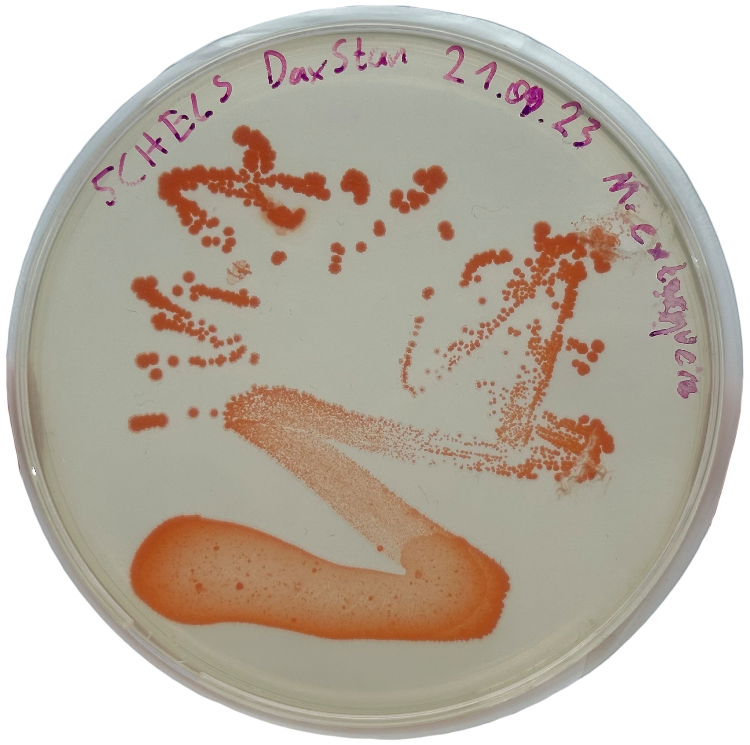
\includegraphics[width=0.8\textwidth]{./media/images/mextorquens_sealed}
    \caption{\emph{M. extorquens} in a sealed petri dish.}
    \label{fig:mextorquens_petri_sealed}
\end{figure}


\section{Methanol Metabolism}
Methylorubrum Extorquens exhibits the ability to utilize the simple alcohol Methanol
CH3OH as its only source of carbon and energy. This metabolism is explained in three
steps:

\begin{enumerate}
    \item \textbf{Initiation: Oxidation of Methanol}
    \begin{itemize}
        \item Location: Periplasm (the space between the inner and outer cell membranes)
        \item Enzymes:
        \begin{itemize}
            \item Methanol dehydrogenase (MposX):
            \begin{itemize}
                \item XoxF1: Requires lanthanides for activity, oxidizing methanol to
                formaldehyde (HCHO) and releasing H+.
                \item XoxF2: Less dependent on lanthanides, potentially involved in
                regulating methanol uptake.
            \end{itemize}
        \end{itemize}
        \item Importance: Formaldehyde is a toxic intermediate, requiring rapid conversion for M. extorquens' survival.
    \end{itemize}
    \begin{figure}[H]
        \centering
        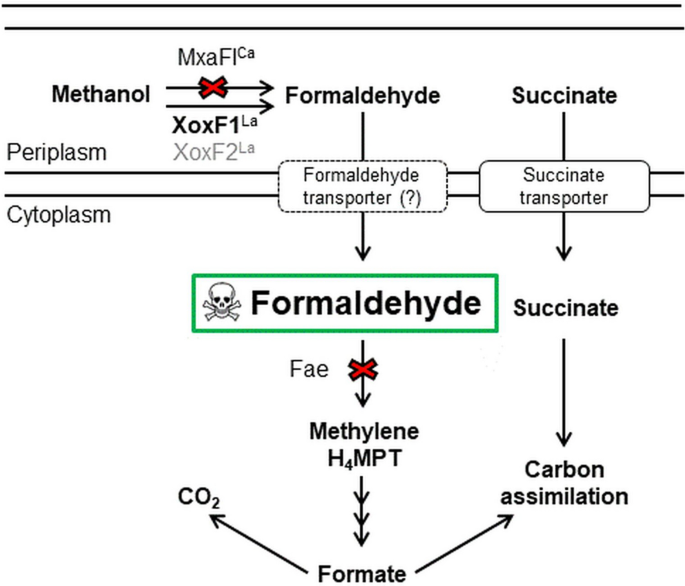
\includegraphics[width=0.8\textwidth]{./media/images/mextorquens_metabolism_methanol}
        \caption{Schematic of the metabolic processes to oxidizing methanol to formaldehyde which is reduced or eliminated and used for growth by cells.}
        \label{fig:mextorquens_metabolism_methanol}
    \end{figure}
    \item \textbf{Capturing the Essence: Fixation of Formaldehyde}
    \begin{itemize}
        \item Molecule: Dephosphotetrahydromethanopterin (dH4MPT) acts as a one-carbon
        carrier.
        \item Enzyme: Formaldehyde-activating enzyme (Fae) catalyzes the reaction, attaching
        formaldehyde to dH4MPT.
        \item Significance: Enables the transport of formaldehyde into the cytoplasm for
        further metabolism.
    \end{itemize}
    \item \textbf{Carbon Assimilation: The Serine Cycle Takes Over}
    \begin{itemize}
        \item Location: Cytoplasm
        \item Pathway:
        \begin{enumerate}
            \item Formate dehydrogenase:
            Oxidizes the formaldehyde-dH4MPT complex, generating formate (HCOO).
            \item Formate acetyltransferase:
            Condenses formate with acetyl-CoA, forming S-acetyl-CoA.
            \item Serine hydroxymethyltransferase: Transfers the one-carbon unit from Sacetyl-CoA to glycine, forming serine.
            \item Serine transaminase: Converts serine to pyruvate, a key metabolic
            intermediate.
        \end{enumerate}
        \item Importance: The serine cycle efficiently converts the one-carbon unit from
        methanol into usable cellular building blocks~\cite{methanol_metabolism}.
    \end{itemize}
    \begin{figure}[H]
        \centering
        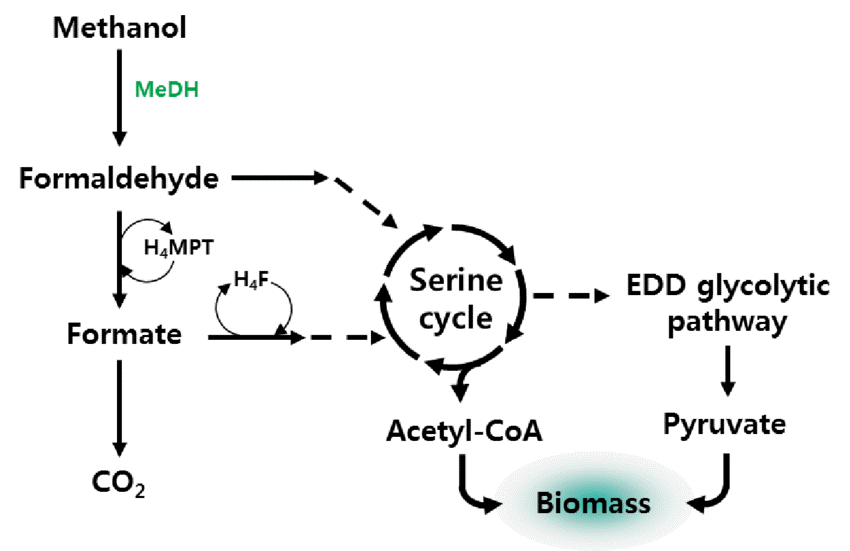
\includegraphics[width=0.9\textwidth]{./media/images/mextorquens_metabolizing_methanol}
        \caption{\emph{Methylorubrum extorquens} metabolizing methanol}
        \label{fig:mextorquens_metabolizing_methanol}
    \end{figure}
\end{enumerate}


\section{Growth}
Methylorubrum Extorquens thrives at temperatures between 30°C and 35°C, making it a
mesophilic bacteria. To promote its optimal growth, the bacteria was placed in a swivel
incubator set to this temperature. Additionally, the nutrient solution needs to be slightly
acidic to neutral, with a pH range of 6.5-7.5, to further enhance growth. Because M.
Extorquens is an aerobic bacteria, the solution in which it is cultivated must be able to
exchange gas and absorb oxygen. This was achieved by sealing the Erlenmeyer flask with
a piece of sterile cotton that allows oxygen to pass through while keeping other bacteria
and fungus out.

Preparation of solid nutrient solution for petri dishes:
\textbf{Materials:}
\begin{itemize}
    \item Peptone 2,5g
    \item Meat Extract 1,5g
    \item Agar 7,5g
    \item \ce{H2O} 500mL
    \item Scale
    \item Autoclave bottle
    \item Spatula
\end{itemize}

\textbf{Execution}
\begin{itemize}
    \item Weigh all the necessary ingredients
    \item Fill the autoclave bottle with around 100ml of water
    \item Add the dry ingredients to the autoclave bottle
    \item Mix the dry ingredients with water
    \item Add the remaining water to the bottle
    \item Shake until mixed
\end{itemize}

Finalizing the solid nutrient solution to be poured into petri dishes:
\textbf{Materials:}
\begin{itemize}
    \item Petri dishes
    \item Autoclave
    \item Autoclave indicator tape
    \item Sterile workbench
\end{itemize}

\textbf{Execution:}
\begin{itemize}
    \item Add a piece of indicator tape on the cap of the autoclave bottle
    \item Autoclave the nutrient solution at 121°C and 1 bar for 15 minutes
    \item After autoclaving the nutrient solution swiftly pour it into the petri dishes
    \item Leave the nutrient solution to harden
    \item Flip the petri dishes carefully on their cover and put them in the fridge
\end{itemize}

\begin{figure}[H]
    \centering
    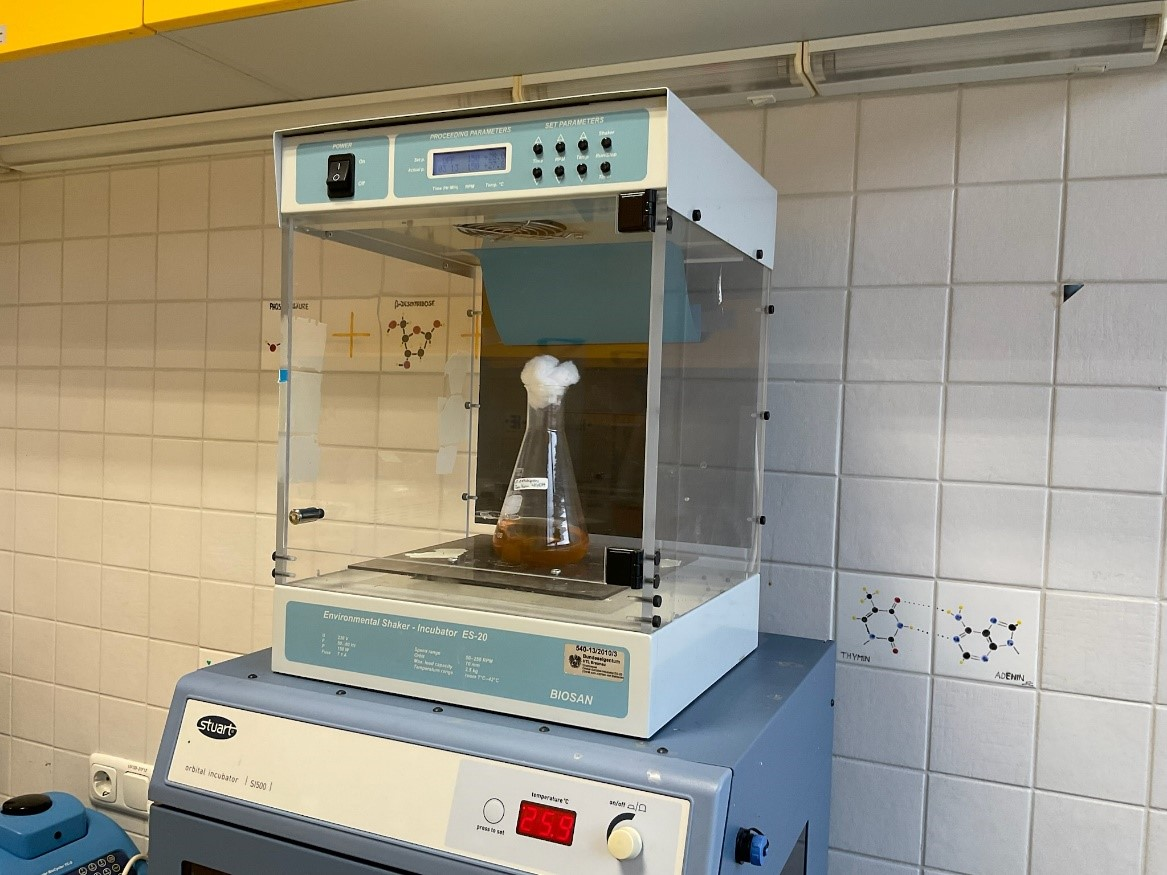
\includegraphics[width=0.9\textwidth]{./media/images/swivel_incubator}
    \caption{Swivel incubator with temperature control used for cultivating \emph{M. extorquens}.}
    \label{fig:swivel_incubator}
\end{figure}

Under optimal conditions, the exponential growth phase of M. Extorquens typically lasts
6-8 hours, during which the number of cells increases rapidly. However, this growth
phase comes to a halt due to a lack of nutrients or waste product accumulation, resulting
in the stationary phase. After this point, the viability and number of cells gradually
decrease, known as the death phase.


\section{Lysis}\label{sec:me_lysis}
In order to obtain Lanmodulin and REE's, it is necessary to break open the cell walls of
the bacteria. This process, known as Lysis, can be accomplished using a variety of
techniques - either mechanical or enzymatic. Mechanical methods include bead beating,
French press lysis, and shock freezing, while enzymatic lysis can be achieved through
Lysozyme treatment, which utilizes an enzyme that specifically breaks down bacterial cell
walls. For this project, a combination of shock freezing and cell wall disruption using an
ultrasonic bath was selected.



